\chapter{实验结果与分析}\label{chap:experiments}
\DemoNotice
\section{实验设置}
本例在第~\ref{chap:data}~章给定的划分上运行四个透明基线。
持续值预测直接使用前一观测；滑动平均取过去九个观测的均值；
岭回归使用相同输入窗口；最后一项在岭回归分数上增加 $\rho=0.2$ 的 EWMA。
所有阈值均由各自的正常校准分数估计，测试标签不参与该过程。

\begin{table}[htbp]
\centering
\gzucaption{实验参数与数据使用范围}{Experimental parameters and permitted data usage}
\label{tab:parameters}
\begin{tabularx}{\textwidth}{@{}lllX@{}}
\toprule
类别 & 参数 & 取值 & 说明 \\
\midrule
数据 & 随机种子 & 20261116 & 每架次使用基础种子加架次编号 \\
输入 & $L,C$ & 9，6 & 一步预测，不跨架次滑窗 \\
训练 & $\lambda$ & 1.0 & 不惩罚截距，目标为残差平方和 \\
校准 & $q$ & 0.99 & 正常校准分数，线性插值分位数 \\
平滑 & $\rho$ & 0.2 & 每架次重置状态 \\
评价 & 点调整 & 不使用 & 按有效目标时刻逐点计算 \\
\bottomrule
\end{tabularx}
\end{table}

\section{总体检测结果}
表~\ref{tab:results} 的数值来自生成脚本，而不是手工指定。
P、R、F1 和 FAR 以百分数表示，AUROC 使用 $[0,1]$ 范围。
本例共有 \DemoTestWindows{} 个有效测试目标，其中
\DemoPositivePoints{} 个被生成器标记为异常。

\begin{table}[htbp]
\centering
\gzucaption[合成实验结果]{四种基线在合成测试集上的逐点检测结果}
 {Pointwise detection results of four baselines on the synthetic test set}
\label{tab:results}
\begin{tabular}{@{}lrrrrr@{}}
\toprule
\multirow{2}{*}{方法} & \multicolumn{3}{c}{逐点检测（\%）} & \multicolumn{2}{c}{补充指标} \\
\cmidrule(lr){2-4}\cmidrule(l){5-6}
 & P & R & F1 & FAR（\%） & AUROC \\
\midrule
\ExampleResultRows
\bottomrule
\end{tabular}
\end{table}

岭回归加平滑的 F1 为 \DemoFone\%，误报率为 \DemoFAR\%。
这些结果并不构成“平滑一定提高检测性能”的证明。
不同基线使用不同分数分布和对应阈值；统一分位数并不意味着统一的测试误报预算。
对固定数据的一次运行也不足以建立具有统计保证的模型排序。

\begin{table}[htbp]
\centering
\gzucaption{结果对应的混淆矩阵计数}{Confusion-matrix counts underlying the reported metrics}
\label{tab:confusion}
\begin{tabular}{@{}lrrrr@{}}
\toprule
方法 & TP & FP & TN & FN \\
\midrule
\ExampleConfusionRows
\bottomrule
\end{tabular}
\end{table}

表~\ref{tab:confusion} 提供原始计数，读者可利用式~\eqref{eq:metrics}
独立复算关键指标。报告计数能够避免百分数四舍五入造成的表面矛盾，
也能说明相同的 F1 可能对应不同的误报和漏报结构。

\section{预测曲线与异常区间}
图~\ref{fig:prediction} 展示 F10 架次中漂移附近的观测和岭回归预测。
两条曲线的接近程度表示局部预测误差，但不能仅凭肉眼判断完整序列的检测效果。
特别是持续偏置进入输入窗口后，预测器可能逐渐追随异常观测。

\begin{figure}[htbp]
\centering
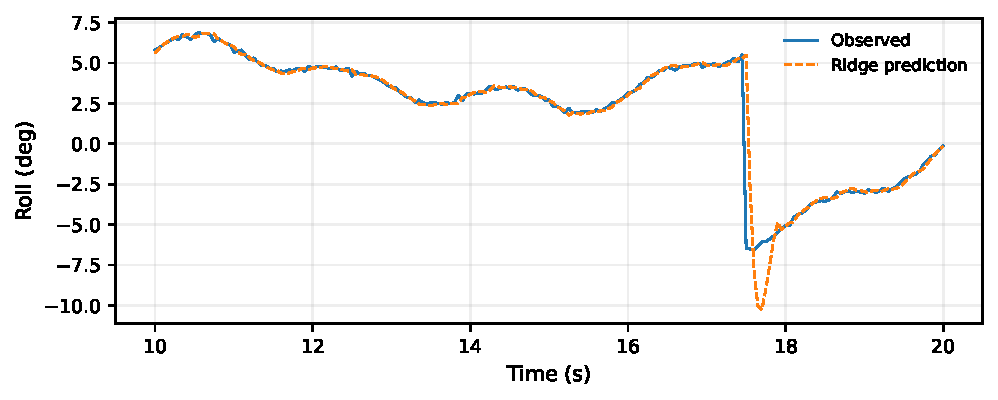
\includegraphics[width=.94\textwidth]{prediction.pdf}
\gzucaption{漂移区间附近的观测与预测}{Observed and predicted roll values near the drift interval}
\label{fig:prediction}
\end{figure}

\begin{figure}[htbp]
\centering
\begin{subfigure}{.48\textwidth}
  \centering
  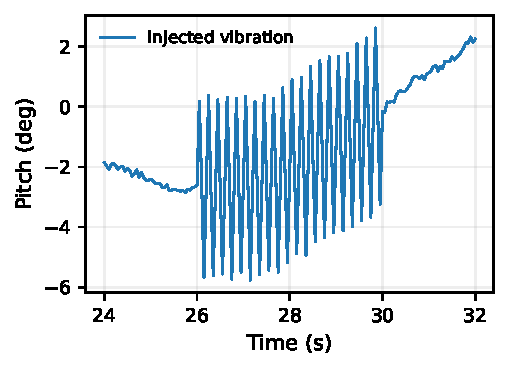
\includegraphics[width=\linewidth]{pitch-event.pdf}
  \caption{俯仰振动}\label{fig:pitch-sub}
\end{subfigure}\hfill
\begin{subfigure}{.48\textwidth}
  \centering
  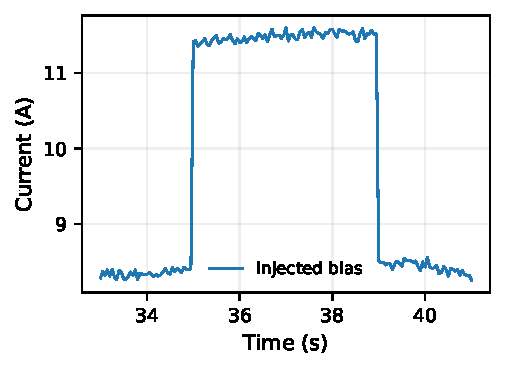
\includegraphics[width=\linewidth]{current-event.pdf}
  \caption{电流偏置}\label{fig:current-sub}
\end{subfigure}
\gzucaption{两类不同的合成异常片段}{Two different types of injected synthetic anomalies}
\label{fig:events}
\end{figure}

图~\ref{fig:events} 使用两个子图展示不同信号。
图~\ref{fig:events}\subref{fig:pitch-sub} 为高频振动，
图~\ref{fig:events}\subref{fig:current-sub} 为恒定偏置。
这一引用写法还用于检验子图编号与主图编号是否独立、稳定。
各子图的单独标题采用中文，图组总题注使用双语，未生成重复的插图清单条目。

\section{分数与平滑敏感性}
\begin{figure}[htbp]
\centering
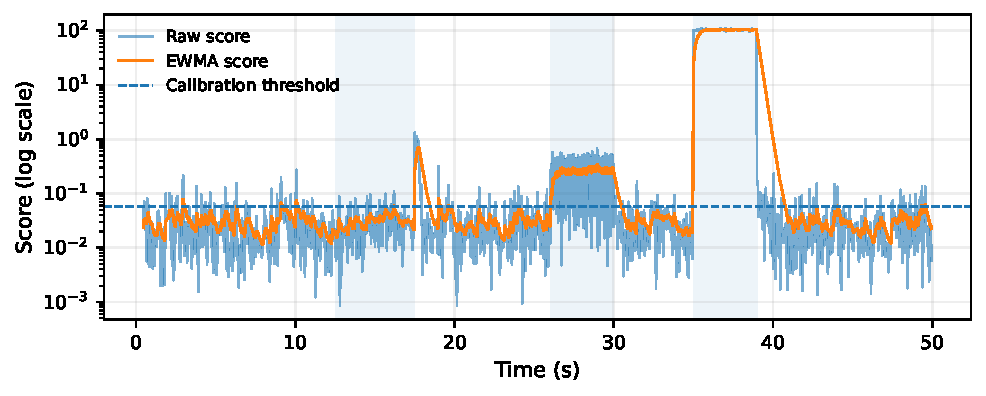
\includegraphics[width=.96\textwidth]{anomaly-score.pdf}
\gzucaption{原始残差、平滑分数与校准阈值}{Raw residuals, smoothed scores, and calibration threshold}
\label{fig:score}
\end{figure}

图~\ref{fig:score} 使用对数纵轴，同时绘出原始分数、平滑分数和固定阈值。
浅色区间表示生成器记录的异常位置，而不是模型预测。
平滑可以改变局部峰值，也会在异常结束后保留历史响应。
因此，在依赖持续观测的检测任务中，减少孤立峰值和增加响应延迟往往同时存在。

\begin{table}[htbp]
\centering
\gzucaption{平滑系数的敏感性分析}{Sensitivity analysis of the smoothing coefficient}
\label{tab:sensitivity}
\begin{tabular}{@{}rrrrr@{}}
\toprule
$\rho$ & P（\%） & R（\%） & F1（\%） & FAR（\%） \\
\midrule
\ExampleSensitivityRows
\bottomrule
\end{tabular}
\end{table}

\begin{figure}[htbp]
\centering
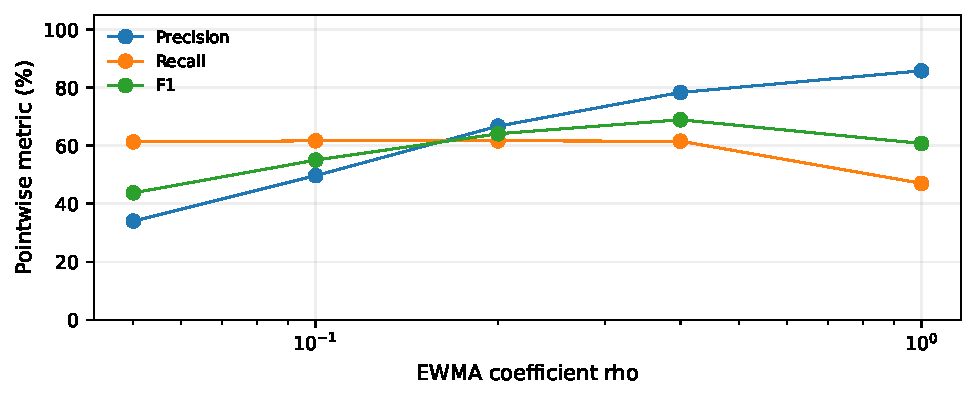
\includegraphics[width=.90\textwidth]{smoothing-sensitivity.pdf}
\gzucaption{不同平滑系数下的逐点指标}{Pointwise metrics under different smoothing coefficients}
\label{fig:sensitivity}
\end{figure}

表~\ref{tab:sensitivity} 和图~\ref{fig:sensitivity} 遍历预先指定的五个系数，
每个系数都重新使用校准数据估计阈值。本节是事后描述，不使用测试结果重新选定默认值。
若将该分析转换为正式模型选择，应再设置独立验证协议，而不能把测试集同时作为调参集。

\section{局限与结果解释}
首先，生成器只模拟少量连续信号与简单耦合，不包括传感器同步误差、
控制器闭环响应或真实故障的传播过程。其次，三次测试飞行共享同一类异常注入规则，
不能代表跨平台泛化。再次，没有重复运行多个随机种子，因而未报告均值和标准差。

最后，本文没有训练 LSTM、PatchTST、Anomaly Transformer 或 MOMENT。
这些模型仅在相关工作中被引用，不能将文献名称填入本例结果表并赋予虚构成绩。
需要比较这些方法时，应实现相同的数据协议、重新训练或按照公开模型的使用规则运行，
并在论文中区分原文结果、复现结果和本文结果。
